% ============================================================
%  CHAPITRE 2 — Section : Modélisation du système
% ============================================================

\section{Modélisation du système}
\label{sec:modele}

L'évaluation des stratégies de gestion d'énergie requiert au préalable un modèle du système suffisamment fidèle pour reproduire les flux de puissance et l'évolution des organes de stockage, mais suffisamment léger pour être simulé sur plusieurs décennies. Cette section précise le modèle macroscopique retenu~: les équations d'évolution de l'état du système d'une part, les profils de puissance qui en constituent les sollicitations d'autre part. L'architecture du micro-réseau a été présentée au chapitre précédent et n'est pas reprise ici~: champ photovoltaïque, batterie lithium-ion et chaîne hydrogène (pile à combustible et électrolyseur) interconnectés autour d'un bus continu commun, en site isolé à La Réunion. Son dimensionnement nominal est simplement rappelé au Tableau~\ref{tab:system_parameters} (section~\ref{sec:ems}).

% ------------------------------------------------------------
\subsection{Équations d'évolution de l'état du système}
\label{subsec:eqs_evolution}
% ------------------------------------------------------------

L'état du système est décrit par deux grandeurs~: l'état de charge $\mathrm{SoC}$ de la batterie et l'énergie $E_{\text{H2}}$ [J] stockée sous forme d'hydrogène. Entre les instants $t$ et $t+\Delta t$, leurs évolutions sont régies par les bilans suivants~:
\begin{equation}
    \label{eq:soc_evol_sys}
    \mathrm{SoC}(t+\Delta t) = \mathrm{SoC}(t) - \frac{P_{\text{bat}}(t)\,\Delta t}{E_{\text{bat,nom}}}\,\eta_{\text{bat}}^{\,k}
\end{equation}
\begin{equation}
    \label{eq:eh2_evol_sys}
    E_{\text{H2}}(t+\Delta t) = E_{\text{H2}}(t) - \Big( P_{\text{ELY}}(t)\,\eta_{\text{ELY}}(t) + \frac{P_{\text{FC}}(t)}{\eta_{\text{FC}}(t)} \Big)\,\Delta t
\end{equation}
où $P_{\text{bat}}$ [W] est la puissance de la batterie, comptée positive en décharge, $E_{\text{bat,nom}}$ [J] son énergie nominale, et $\eta_{\text{bat}}^{\,k}$ son rendement, avec $k=1$ en charge et $k=-1$ en décharge. Ce rendement est ici supposé constant et égal à $0{,}95$. Du côté hydrogène, $P_{\text{ELY}}$ [W] est la puissance de l'électrolyseur, négative par nature puisqu'il ne peut que consommer, et $P_{\text{FC}}$ [W] celle de la pile à combustible, positive par nature puisqu'elle ne peut que produire~; $\eta_{\text{ELY}}$ et $\eta_{\text{FC}}$ sont leurs rendements respectifs, qui dépendent du point de fonctionnement~\cite{lu_optimization_2023}\cite{jia_novel_2023}.

Ces rendements sont implémentés sous forme de tables de correspondance exprimant le rendement de conversion en fonction de la puissance relative de fonctionnement. Ce choix présente un intérêt particulier au regard du vieillissement~: lorsqu'un composant vieillit, sa puissance maximale délivrable diminue, de sorte que fournir une même puissance absolue correspond à une charge \emph{relative} plus élevée, et donc à un point différent le long de la courbe de rendement. La perte d'efficacité associée au vieillissement est ainsi capturée implicitement par ce déplacement du point de fonctionnement dans la table, qui se traduit par une consommation d'hydrogène accrue à service équivalent à mesure que les composants se dégradent.

À tout instant, le bilan de puissance sur le bus continu assure la conservation de l'énergie~:
\begin{equation}
    \label{eq:power_balance_sys}
    P_{\text{Load}} - P_{\text{PV}} = P_{\text{FC}} + P_{\text{ELY}} + P_{\text{bat}}
\end{equation}
où $P_{\text{Load}}$ [W] est la puissance consommée par les usagers (positive) et $P_{\text{PV}}$ [W] la puissance fournie par les panneaux (positive). Ces deux valeurs peuvent différer des trajectoires planifiées $\hat{P}_{\text{Load}}$ et $\hat{P}_{\text{PV}}$ issues des profils~: un tel écart apparaît, par exemple, lorsque la demande ne peut être satisfaite par les composants ou lorsqu'un écrêtage est réalisé.

Dans cette formulation, les variables de contrôle du système sont les trois puissances $P_{\text{bat}}$, $P_{\text{FC}}$ et $P_{\text{ELY}}$~; il s'agit donc d'un problème de commande à trois dimensions. Une fois ces trois puissances déterminées par l'EMS, le bilan global~\eqref{eq:power_balance_sys} est évalué et peut, le cas échéant, s'écarter de la trajectoire de référence~: cette latitude permet au système de \emph{ne pas} suivre exactement la demande à certains instants lorsque la réduction de la dégradation est jugée prioritaire. Les contraintes opérationnelles (puissances maximales des composants, bornes de SoC, capacité du réservoir d'hydrogène) sont respectées lors de cette allocation, comme détaillé dans l'algorithme de simulation (section~\ref{sec:simulation}).

% ------------------------------------------------------------
\subsection{Profils de puissance}
\label{subsec:profils}
% ------------------------------------------------------------

Les sollicitations du système sont entièrement déterminées par deux profils temporels~: la production photovoltaïque $\hat{P}_{\text{PV}}$ et la demande de charge $\hat{P}_{\text{Load}}$. Ces profils ne sont pas synthétiques~: ils proviennent de données de terrain fournies par le concepteur du micro-réseau à La Réunion. Aucun modèle de conversion irradiance-puissance (inclinaison des panneaux, conversion du rayonnement global horizontal, etc.) n'intervient donc~: le profil PV est directement issu de mesures de production sur site, tandis que le profil de charge résulte d'enquêtes de terrain sur les habitudes de consommation des résidents locaux, agrégées pour constituer un profil de consommation représentatif (Figure~\ref{fig:profiles}).

\begin{figure}[h!]
    \centering
    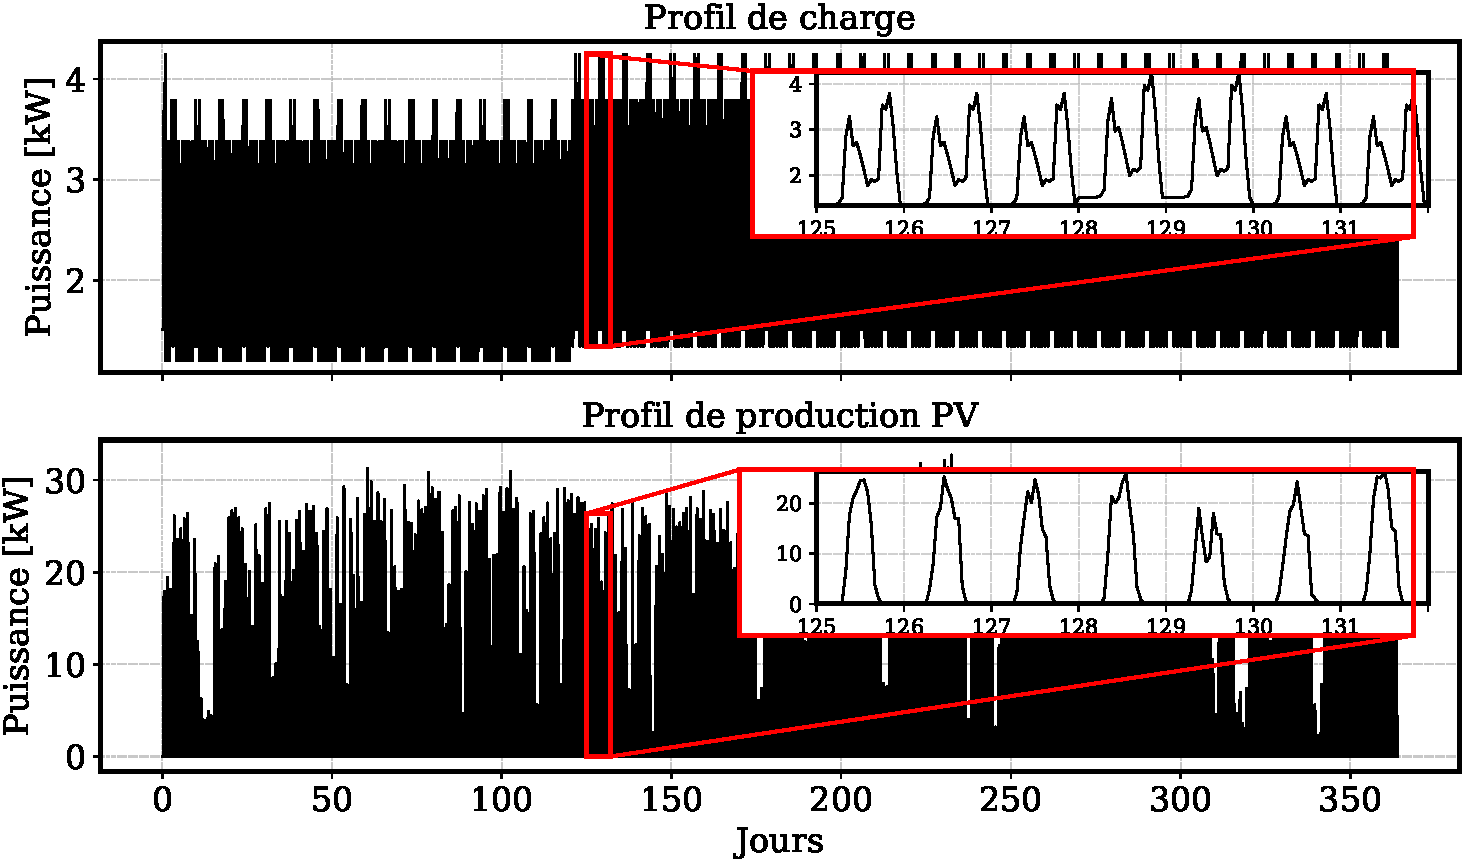
\includegraphics[width=\linewidth]{Chapitre 2/Modele/Figures/sidelec_conso_PV_fr.pdf}
    \caption{Profils de puissance utilisés en simulation~: charge et production photovoltaïque }
    \label{fig:profiles}
\end{figure}
\FloatBarrier

Deux caractéristiques de ces profils méritent d'être soulignées, car elles conditionnent l'interprétation des résultats. D'une part, la production PV est nettement surdimensionnée relativement à la demande moyenne~: la puissance crête du champ (environ \SI{33}{\kilo\watt}) dépasse largement la charge moyenne (de l'ordre de \SI{2}{\kilo\watt}), ce qui se traduit par d'importants excédents d'énergie en journée, dont l'électrolyseur et la batterie doivent disposer, ou par un niveau important d'écrêtage. D'autre part, en raison de la position quasi équatoriale de l'île, la variabilité \emph{saisonnière} de la ressource solaire comme de la demande est relativement limitée~; les profils mesurés intègrent néanmoins la variabilité réelle, jour après jour et à l'intérieur de chaque journée, de la production et de la consommation du site. Ce contexte (fort excédent PV, faible saisonnalité) est caractéristique du cas d'étude et devra être gardé à l'esprit lors de la généralisation des conclusions à d'autres sites (cf.\ section~\ref{sec:conclusion_chap}).